\chapter{Methodology}
\label{Methodology}
In previous chapters we introduced our research problem, listed and explained the solution options with the theoretical background. In this chapter we shall try to explain our practical approach for carrying out the research along with the software development required to support the experimentation and data analysis for our research. On a practical level following were some major tasks that were required to fulfil scope of our research.
\begin{itemize}
\item Understanding energy efficiency, smart grids and available data.
\item Requirement engineering and use case preparation.
\item Understanding Data Analytics ecosystem, evaluating the big data tools and solutions.
\item Exploratory data analysis and selection of algorithms and data analysis tools with respect to use cases. 
\item Developing an end to end big data analytics platform.
\item Data collection, storage and preprocessing.
\item Use case specific data analysis and evaluation of results.
\item Visualization of results 
\item Documentation of the research, process, software development and results.
\end{itemize}
Some of these tasks were required to be performed in a sequential way e.g. requirement engineering and evaluation of big data tools were required before developing the big data analytics platform or selecting the algorithms. Similarly we need to have results before visualizations could be created. On the other hand some of the tasks could have been executed in parallel. For example the documentation was an ongoing process along with all other tasks. Similarly literature review for understanding each component of our research was also an ongoing process through the time line for this thesis. The regardless of sequential and parallel tasks we need to iterate for continuous improvement.

To tackle these challenges we needed a methodology that can support sequential and parallel task execution with support for iterations to improve. Like most of scientific researches, fail fast and small to succeed was the key for us. In the list of tasks mentioned above. Most of them requires conceptualization and tested quickly using rapid prototyping. Taking it as a software development task initially, we had some candidate models such as water fall model,agile development model, spiral model and incremental model etc. Here we shall briefly discuss the advantages and disadvantages in context to our research project. 
\begin{itemize}
\item \textbf{Waterfall model} offered the simplest approach of requirement engineering, design, implement, test and operate our research. How ever it is inherently sequential and had weak support for iterations.
\item \textbf{Agile development model} Agile methodology\cite{martin2003agile} is rapid, iterative and supports quick prototyping but it requires additional communication and management overhead like scrum meetings. Managing it along with stakeholders like VTT and CIVIS projects was very hard.
\item \textbf{Spiral Model} is a risk driven process model.It supports prototyping, provides good way of avoiding major failure risks, it is iterative. However it needs a lot of resources during planning phase specially when the spiral keeps growing in size. It is usually very successful for large projects but it has over heads for small projects like our thesis research. We shall be discussing more about using parts of the spiral model later in this chapter.
\item \textbf{Incremental model} relies on small incremental steps with each step consist of independent design, implement and test phase. In the begining, Incremental model was the best fit among other candidate models for our thesis research.We were able to prototype small functional units of the big data analytics platform very quickly while independently working on the use cases. However during platform development and data analysis part. It has started creating integration over heads. For example integrating two different data processing tools together for a single use case becomes difficult  when they were configured in two different incremental steps.  
\end{itemize}
Learning from the problems that we face from  incremental model we altered our approach to adapted version of another very flexible software research and development methodology known as ``Kumiega-Van Vliet Trading System Development Methodology''\cite{kumiega2008software}.

\section{Kumiega-Van Vliet Model}   
      
Kumiega-Van Vliet Trading System Development Methodology \((K|V)\) was developed in 2008 for software development required specifically for trading systems. It is the combination of three general purpose software and new product development models i.e. waterfall model, spiral model and stage gate model. We have already explained the waterfall and spiral models. Stage gate model consists of stages e.g. scoping, development, implementation, testing etc. Each stage or combination of stages can be controlled with an approval gate. Process can not move from a stage to other stage if the gate in between them is not approved.This model provides a good control over the development model to ensure quality. However it may cause delays because of the organizational hierarchies dictating the gates.

 \((K|V)\) model tries to overcome the short comings of these three models by combining them to a single paradigm for trading system development\cite{kumiega2008software}. In spiral model in start smaller time is allocated to four basic steps i.e. research planning implementation and test. These four steps can be performed again and again in cycles. To avoid spiral to grow two much after each cycle a stage gate controls if process can be passed to next stage or it needs to be sent back to perform another cycle in same stage. Just like waterfall there can be number of stages. But for continuous improvements process there is an iteration channel available unlike traditional waterfall model.
 \section{Adaptation of Kumiega- Van Vliet Model}
 \begin{figure}[ht]
   \begin{center}
     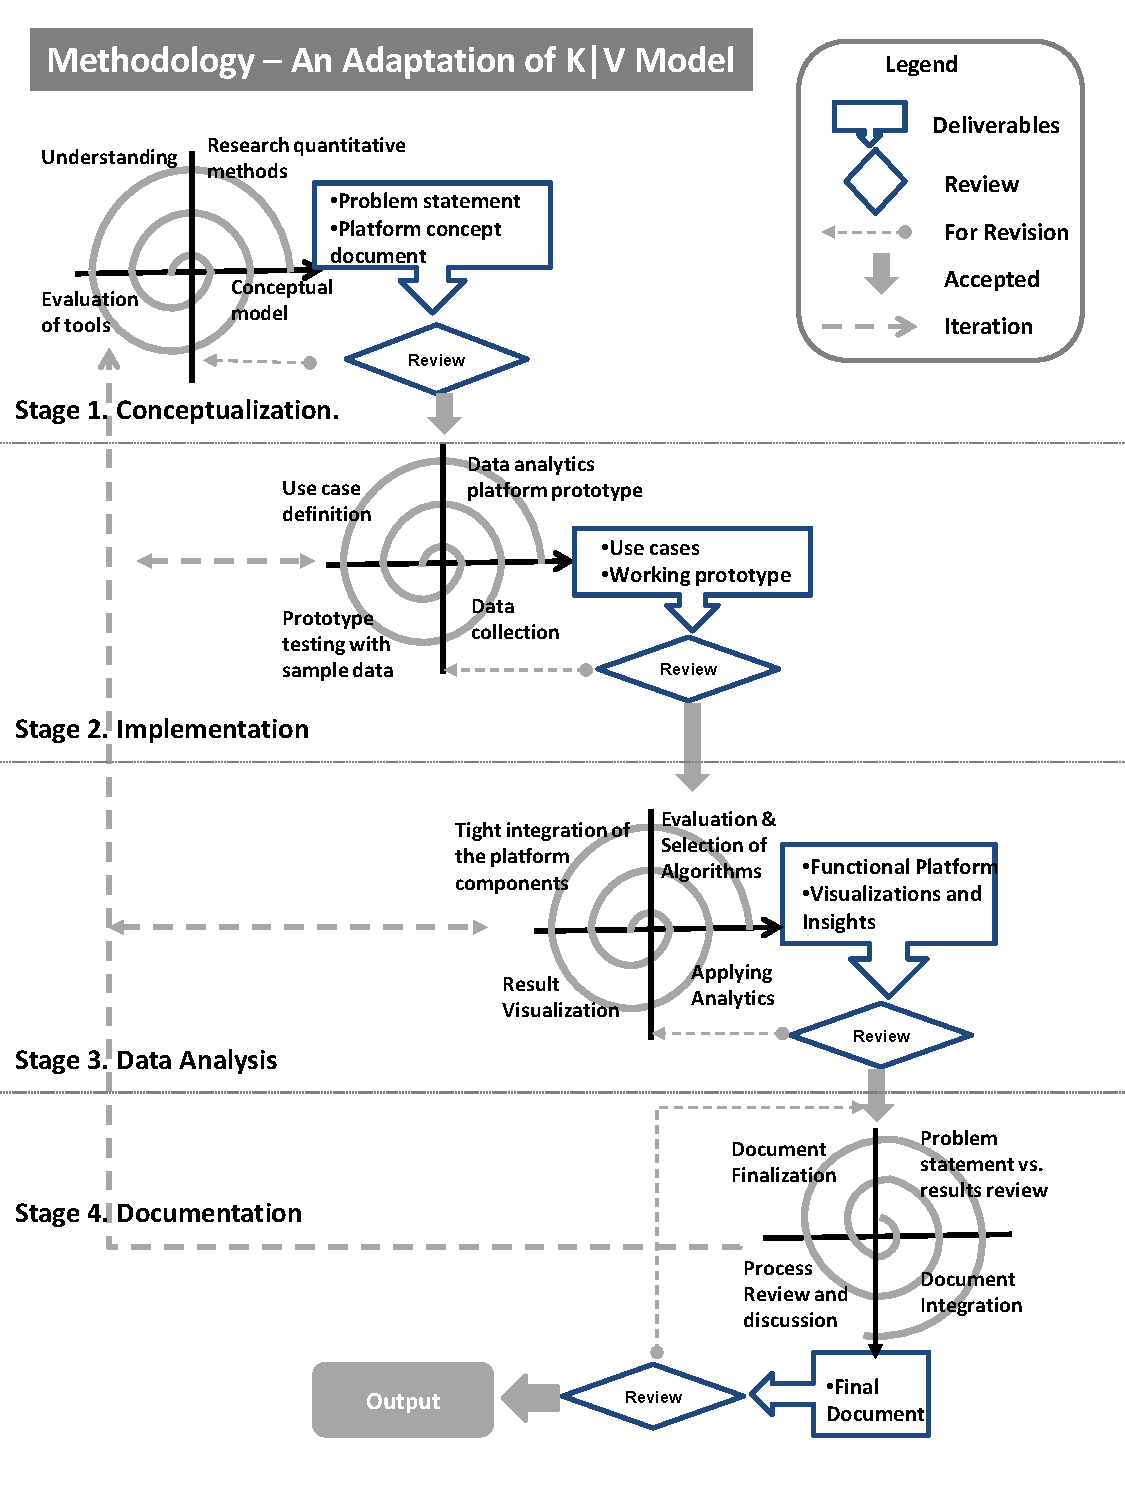
\includegraphics[width=\textwidth]{images/kv_method.pdf}
     \caption{Methodology, An Adaptation of K|V Model}
     \label{fig:kv}
   \end{center}
 \end{figure}  
